\documentclass{article}
    \usepackage{amsmath}
    \usepackage{graphicx}
    \usepackage{titlesec}
    \usepackage{verbatim}
    \usepackage{color}
    \usepackage{framed}
    
    \usepackage{hyperref}
    
    \graphicspath{ {Pic/} }

    \usepackage{HandoutTemplate}
    \usepackage{xcolor}
    \hypersetup{
    	colorlinks=true,
    	linkcolor={red!50!black},
    	citecolor={green!40!black},
    	urlcolor={green!40!black}
    }
    
    % ------- Text Formating ------- %
    \settextfont[Scale=1.1]{XB Zar}
    \setlatintextfont{Linux Libertine}
    % \setdigitfont{Linux Libertine}
    
    \renewcommand{\baselinestretch}{1.7}
    \setlength{\parindent}{1.5em}
    

    % ------- Section Formatting ------- %
    \titleformat{\section}
        {\normalfont\Large\bfseries}
        {\thesection}
        {1em}
    {}
    

    % ------- Math Formatting ------- %
    \DefaultMathsDigits
    \DeclareMathOperator{\var}{Var}


    % ------- Code Formatting ------- %
    \definecolor{shadecolor}{gray}{0.95}
    
    \newenvironment{changemargin}[2]
    {%
    \begin{list}{}{%
      \setlength{\topsep}{0pt}%
      \setlength{\leftmargin}{#1}%
      \setlength{\rightmargin}{#2}%
      \setlength{\listparindent}{\parindent}%
    %   \setlength{\itemindent}{\parindent}%
      \setlength{\parsep}{\parskip}%
    }%
    \item[]
    }
    {
        \end{list}
    }


    \newenvironment{code}
        {\LTR\snugshade\verbatim}
        {\endverbatim\endsnugshade\RTL}
  
    \newcommand{\inlineCode}[1]{\lr{\colorbox{lightgray!20}{\texttt{#1}}}}
    
    \begin{document}
    \handout
    {\lr{CE-40443}}
    {}
    {پاییز ۱۳۹۷}
    {پیاده‌سازی شبکه‌ی \lr{P2P}}
    {۱ بهمن، ساعت ۵ صبح}
    
    \vspace{0.3cm}
     
\section{چکیده}

   هدف این پروژه پیاده‌سازی یک شبکه‌ی \lr{Peer to Peer} و واسط کاربری برای ارتباط با شبکه است.  این شبکه شامل دو جز اصلی است: 

\begin{itemize}
   \item   	یک \lr{Root} که در نقش \lr{DNS} عمل می‌کند.

\item تعدادی \lr{Node}‌ که به صورت گراف همبند بدون دور (درخت) با ریشه‌ی \lr{Root} به یک‌دیگر وصل شده و تشکیل شبکه می‌دهند.
   برنامه‌ی نوشته شده باید قابلیت اجرا شدن هم در نقش \lr{Root} و هم در نقش \lr{Peer} را داشته باشد و به گونه‌ای طراحی شود که تبادل پیام در شبکه قابل مشاهده باشد.
\end{itemize}
 

	\newpage
\begin{center}
	\vspace*{3cm}
	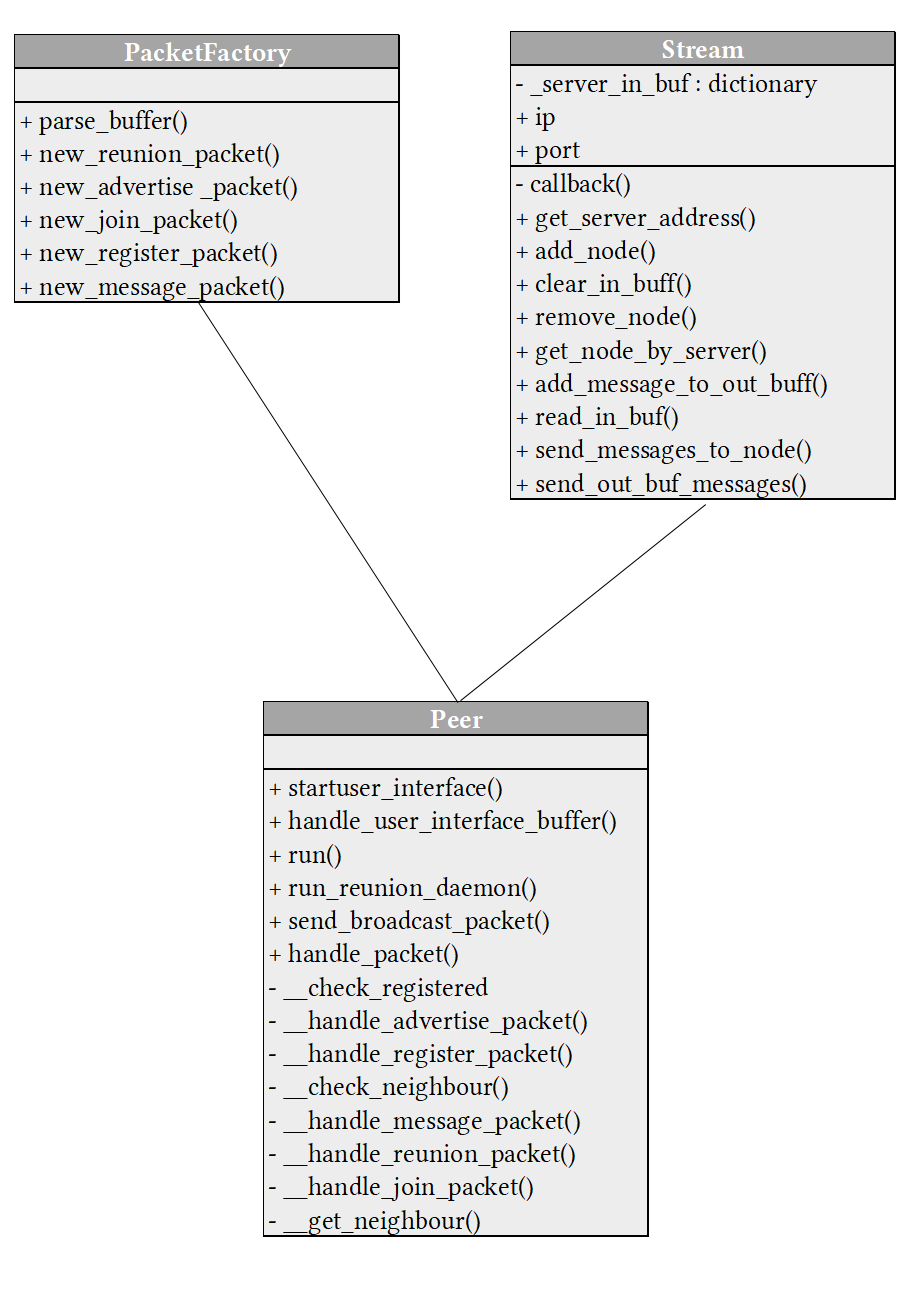
\includegraphics[scale=0.9]{UML1}
\end{center}

\begin{center}
	\vspace*{6cm}
	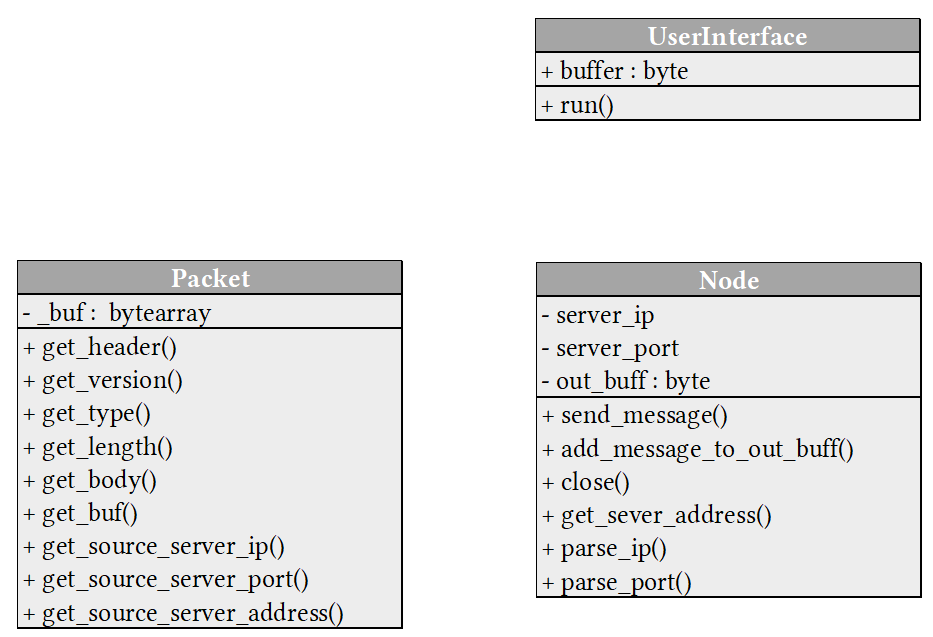
\includegraphics[scale=0.9]{UML2}
\end{center}
	
	


\newpage
\section{مقدمه}
\lr{P2P} یا شبکه‌ی همتا به همتا توزیعی از معماری شبکه‌های کامپیوتری است که در آن هر \lr{Peer} هم نقش \lr{Client} و هم نقش \lr{Server} را بازی می‌کند. و از این طریق می‌تواند به تبادل پیام در شبکه‌ای از \lr{Peer}ها بپردازد. در این نوع شبکه‌ها بر خلاف شبکه‌های \lr{Client-Server}، سرور مرکزی وجود ندارد. \lr{Torrent}، \lr{Tor} و \lr{Bitcoin} مثال‌هایی شناخته شده از شبکه‌های \lr{P2P} هستند. نکته‌ای که حائز اهمیت است آن است که در عمل شبکه‌ای که به طور کامل \lr{P2P} باشد وجود ندارد و حتی در شبکه‌های \lr{P2P} هم \lr{Node}هایی وجود دارد که سبب پابرجایی شبکه هستند و حذف آن‌ها از شبکه سبب اخلال در شبکه می‌شود.



\section{پروتکل شبکه}

\subsection{\lr{Client}}
   اولین گام پس از ورود هر \lr{Client} به شبکه رجیستر شدن آن در شبکه است. برای این کار \lr{Client} با فرستادن پیام \lr{Register Request} به \lr{Root} شبکه خود را در شبکه ثبت می‌کند.\\
   در ادامه هر \lr{Client} باید آدرس \lr{Client} پدر (اولین همسایه‌) را از \lr{DNS} بگیرد. برای این کار \lr{Client} با فرستادن پیام \lr{Advertise} به \lr{Root} درخواست یک آدرس کرده و در جواب آن آدرسی از طرف \lr{DNS} (که در این شبکه همان \lr{Root} است) به \lr{Client} ارسال می‌شود.\\
   حال \lr{Client} با فرستادن پیام \lr{join} به آدرسی که از \lr{Root}‌ دریافت کرده است، درخواست متصل شدن خود را به \lr{Client} مورد نظر اعلام می‌دارد. \lr{Client} پس از اتصال به اولین همسایه‌ی خود، جزئی از شبکه شده و می‌تواند پیام‌های خود را با دیگر کلاینت‌های داخل شبکه در قالب \lr{Broadcast} به اشتراک بگذارد.\\
   هر \lr{Client} موظف است هر ۴ ثانیه یک بار با فرستادن پیام \lr{Reunion Hello} از طریق پدرش به \lr{Root}، و دریافت پاسخ\lr{Reunion Hello Back} از طریق همان مسیر و از طرف \lr{Root}، از اتصال به شبکه اطمینان حاصل نماید.\\
   هر \lr{Client} در صورت دریافت پیام \lr{Reunion Hello}، آدرس خود را به انتهای پیام اضافه، فیلد \lr{Number of Entries} را به روزرسانی کرده و پیام را به پدرش می‌فرستد. همچنین کلاینت‌ها در صورت دریافت پیام\lr{Reunion Hello Back}، آدرس خود را از انتهای پیام برداشته، فیلد \lr{Number of Entries} را به روزرسانی کرده و پیام را به آدرس بعدی می‌فرستند.\\
   در صورتی که پس از مدت زمان معینی (بدست آوردن این زمان به عهده‌ی خودتان است) \lr{Client} پاسخ پیام \lr{Reunion Hello} خود را دریافت نکرد، اتصال خود به شبکه را قطع شده فرض می‌کند و با فرستادن پیام \lr{Advertise Request}، درخواستی مبتنی بر گرفتن آدرسی جدید به \lr{Root} می‌فرستد.\\
   نکته: در این شبکه عمق درخت حداکثر برابر ۸ است.\\
   
   
   
\subsection{\lr{Root}}
اولین وظیفه‌ی \lr{Root} در قبال هر \lr{Client}، ثبت \lr{Client} در شبکه با پاسخ به پیام \lr{Register Request}  فرستاده شده از \lr{Client} است. \\
از دیگر وظایف \lr{Root} فرستادن آدرس یک \lr{Client} (هر \lr{Client} بیشتر از دو فرزند ندارد) به عنوان \lr{Client} پدر در پاسخ پیام \lr{Advertise Request} است.\\
آخرین وظیفه‌ی \lr{Root} انتظار به مدت لازم (بدست آوردن این زمان به عهده‌ی خودتان است) برای دریافت پیام \lr{Reunion Hello} و فرستادن پیام\lr{Reunion Hello Back} در پاسخ پیام دریافتی است. در صورتی که پس از گذشت زمان معین از \lr{Client} پیامی در قالب \lr{Reunion Hello} دریافت نشود، \lr{Root} آن \lr{Client} را حذف شده در نظر گرفته و دیگر آدرس آن \lr{Client} و زیر درخت مربوط به آن را Advertise نمی‌کند.\\




\section{پیاده‌سازی}
در این بخش به معرفی وظایف اشیا ساخته شده از هر کلاس، تابع‌های موجود در آن‌ها و همچنین نحوه گرفتن ورودی در آن‌ها می‌پردازیم.

\subsection{\lr{Peer}}
در این پروژه هر \lr{Node} موجود در شبکه از جنس \lr{Peer} است؛ چه \lr{Client} باشد چه \lr{Root}. به عبارتی ساده‌تر شبکه‌ی پیاده‌سازی شده عملاً اجتماعی از چندین \lr{Peer} است که به نحوی به یکدیگر متصل‌اند (شبکه گرافی همبند است).  \\
\lr{Peer} همچنین وظیفه‌ی تولید \lr{Packet} با استفاده از پیام‌های ورودی \lr{Stream} یا به صورت دلخواه به کمک \lr{PacketFactory} را دارد. تبدیل \lr{Packet} به پیام و تحویل آن به \lr{Stream} جهت ارسال آن در شبکه نیز از وظایف \lr{Peer} می‌باشد. علاوه بر این انجام \lr{action} هر \lr{Packet} به عهده‌ی \lr{Peer} است.




\subsection{\lr{Stream}}   
\lr{Stream} در سطح شبکه پیاده‌سازی شده و مربوط به لایه‌ی کاربردی نیست. وظیفه‌ی اصلی \lr{Stream} ارسال و دریافت پیام‌ها از طریق \lr{Node}های متفاوت ست. مدیریت در خصوص آن که هر \lr{Node} چه پیام‌هایی باید بفرستد، چه پیام‌هایی را از چه \lr{Node}هایی باید دریافت کند و در جواب آن‌ها چه پیام‌هایی را بفرستد، به عهده‌ی \lr{Stream} است. \\
\lr{Stream} با توجه به مقصد پیام، بافر را به \lr{Node} مورد نظر می‌رساند. \lr{Node} پیام را از طریق \lr{Stream} دریافت کرده و با طی روند خاصی پیام را تبدیل به بافر کرده و به \lr{Node} مورد نظر ارسال میکند. از طرفی بافر‌های ورودی هر \lr{Node} را تبدیل به پیام می‌کند و به \lr{Peer} تحویل می‌دهد.




\subsection{\lr{Node}}
\lr{Stream} برای کار با \lr{Peer}های دیگر از \lr{Node} استفاده می‌کند. به بیانی واضح‌تر هر \lr{Stream} شامل تعداد زیادی \lr{Node} می‌شود که هر کدام از این \lr{Node}ها دارای یک سوکت است که این سوکت به سوکت سرور \lr{Peer} دیگر متصل است. هر \lr{Node} دو بافر ورودی و خروجی دارد. در بافر ورودی پیام‌ّهای فرستاده شده و در بافر خروجی پیام‌هایی که باید فرستاده شوند وجود دارند.



\subsection{\lr{Packet}}
تمامی پیام‌هایی که در شبکه انتقال می‌یابند از جنس \lr{Packet} هستند. \lr{Packet} شی‌ای است برای \lr{Peer} قابل فهم است. اما هر \lr{Packet} قبل از انتقال پارس شده و به بافر تبدیل می‌شود و این بافر است که در شبکه انتقال می‌یابد. پس بافری که \lr{Peer} از \lr{Stream} دریافت می‌کند، لازم است به \lr{Packet} تبدیل شود تا قابل فهم شود.
ساختار هر \lr{Packet} در ادامه مشخص شده است:
\begin{itemize}
\newpage
	\item \lr{Register Request}\\\\
		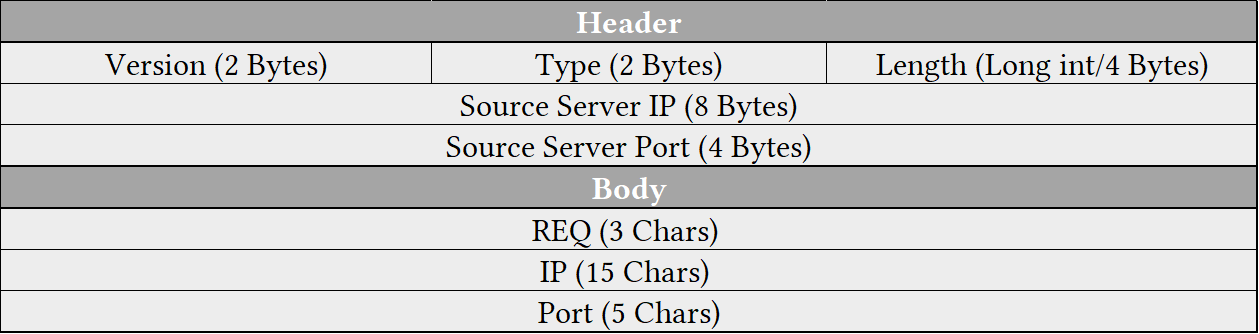
\includegraphics{RegisterRequest}
	\item \lr{Register Response}\\\\
		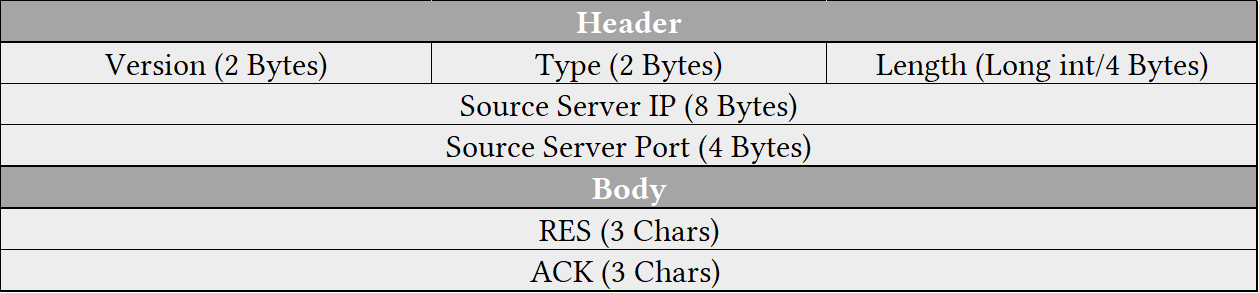
\includegraphics{RegisterResponse}	
	\item \lr{Advertise Request}\\\\
		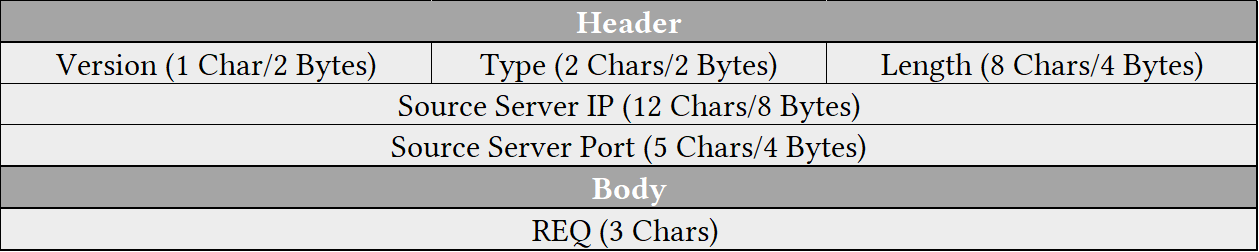
\includegraphics{AdvertiseRequest}	
	\item \lr{Advertise Response}\\\\
		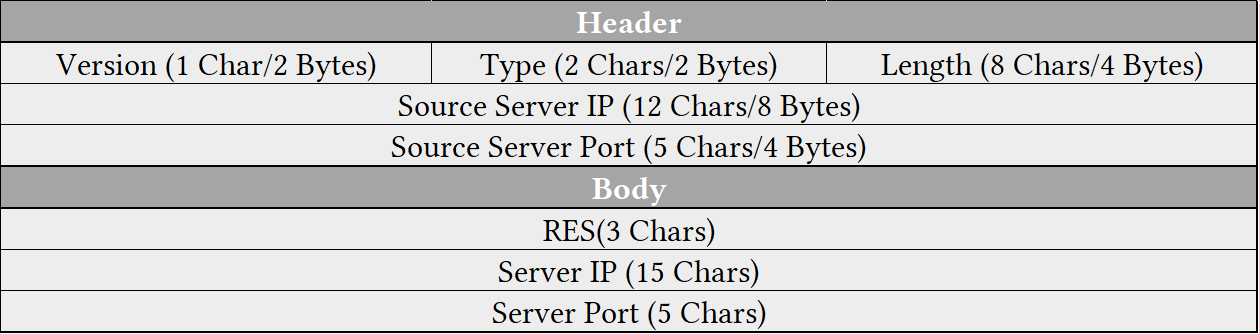
\includegraphics{AdvertiseResponse}	
	\item \lr{Join}\\\\
		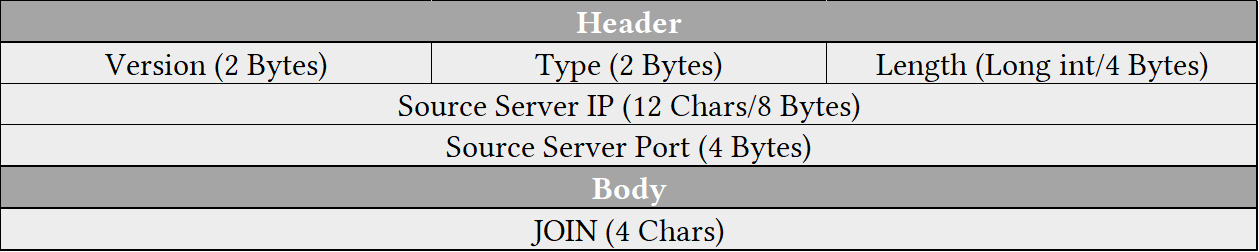
\includegraphics{Join}
	\item \lr{Message}\\\\
		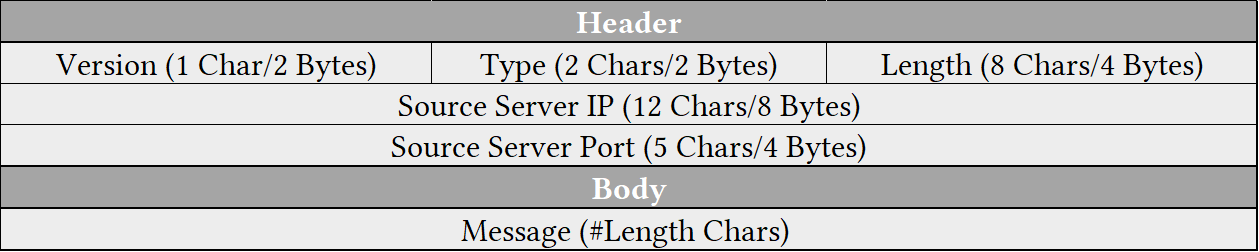
\includegraphics{Message}
	\item \lr{Reunion Hello}\\\\
		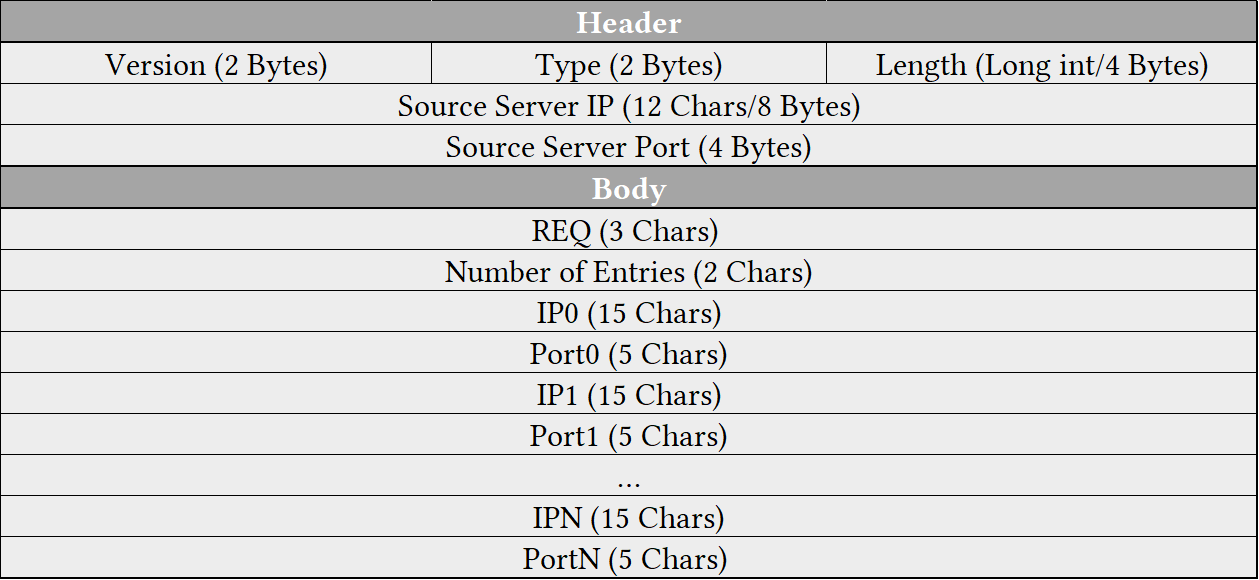
\includegraphics{ReunionHello}	
\newpage
	\item \lr{Reunion Hello Back}\\\\
		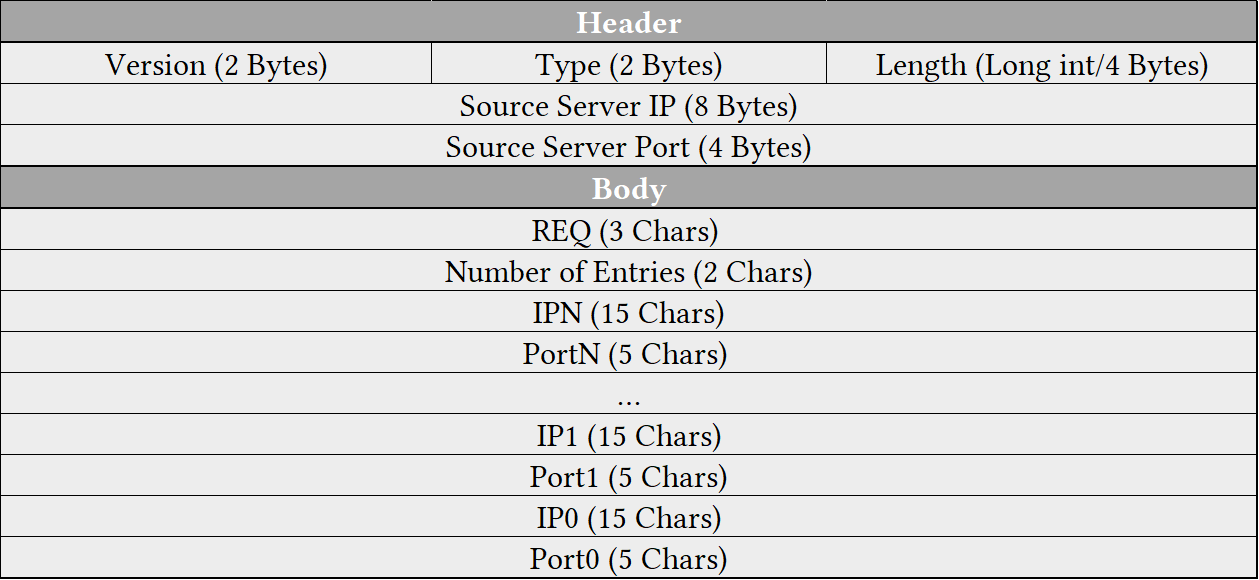
\includegraphics{ReunionHelloBack}	
\end{itemize}



\subsection{\lr{PacketFactory}}
هر \lr{Peer} برای تولید \lr{Packet} به \lr{PacketFactory} نیاز دارد. Packetهای تولید شده، توسط این کلاس به بافر تبدیل شده و برای انتقال از طریق \lr{Peer} به \lr{Stream} داده می‌شود.



\subsection{\lr{UserInterface}}
همان‌طور که از نام این کلاس پیداست، وظیفه‌ی آن ایجاد یک واسط بین برنامه و کاربر است. از طریق این کلاس کاربر می‌تواند عملکرد \lr{Peer} را کنترل کرده و دستور ایجاد \lr{Packet}های متفاوت را بدهد.



\newpage
 \section{نکات دیگر}
    \begin{itemize}
    \item برای پیاده‌سازی پروژه تنها از زبان پایتون می‌توانید استفاده کنید.
    \item گروه‌ها به صورت دو نفره است.
    \item در فایل پیوست تابع‌هایی که برای هر کلاس نیاز است پیاده‌سازی شود، توضیح داده شده است.
    \item فایل‌های تحویل دادنی را به فرمت \lr{.zip} درآورده و در سامانه‌ی کوئرا بارگذاری نمایید.
    \item نام فایل ارسالی باید به فرمت \lr{CN\_Project\_STDID1\#\_STDID2\#} باشد.
    \
	\end{itemize}
    \vfill
    \vspace{1cm}
    $\hfill$ موفق باشید
    \end{document}